\documentclass[letterpaper,12pt]{article}
\usepackage{amsmath}  % improve math presentation
\usepackage{graphicx} % takes care of graphic including machinery
\usepackage{mathrsfs}


\usepackage[final]{hyperref} % adds hyper links inside the generated pdf file
\hypersetup{
	colorlinks=true,       % false: boxed links; true: colored links
	linkcolor=blue,        % color of internal links
	citecolor=blue,        % color of links to bibliography
	filecolor=magenta,     % color of file links
	urlcolor=blue         
}

\title{Eighth Assignment for Computational Physics}
\date{\today}
\author{Xinyu Liu}


\begin{document}
\maketitle
\tableofcontents

\newpage

\section{My Github Page URL}
\url{https://github.com/rising1227/phys-ga2000}

\section{Newman 8.6: Harmonic and anharmonic oscillator}

the associated code can be found at 9-1.phys

In order to solve a second order ODE, we first turn it into a first order equation:

\begin{align}
    & \frac{dx}{dt} = y\\
    & \frac{dy}{dt} = f(x)
\end{align}

\begin{itemize}
    \item In the harmonic oscillator problem, we have $f(x) = -\omega^2 x$.
    \item For anharmonic oscillator in part c, we have $f(x) = -\omega^2 x^3$.
    \item For van der Pol oscillator, we have $f(x) = -\omega^2 x + \mu (1-x^2)*y$
\end{itemize}

In all the problems, we solve the differential equation with 4th order Runge-Kutta method.

First we solve the harmonic trap problem. Here's the result for A = 1.

\begin{table}[!h]
    \centering
    \caption{x as a function of time for harmonic trap}
    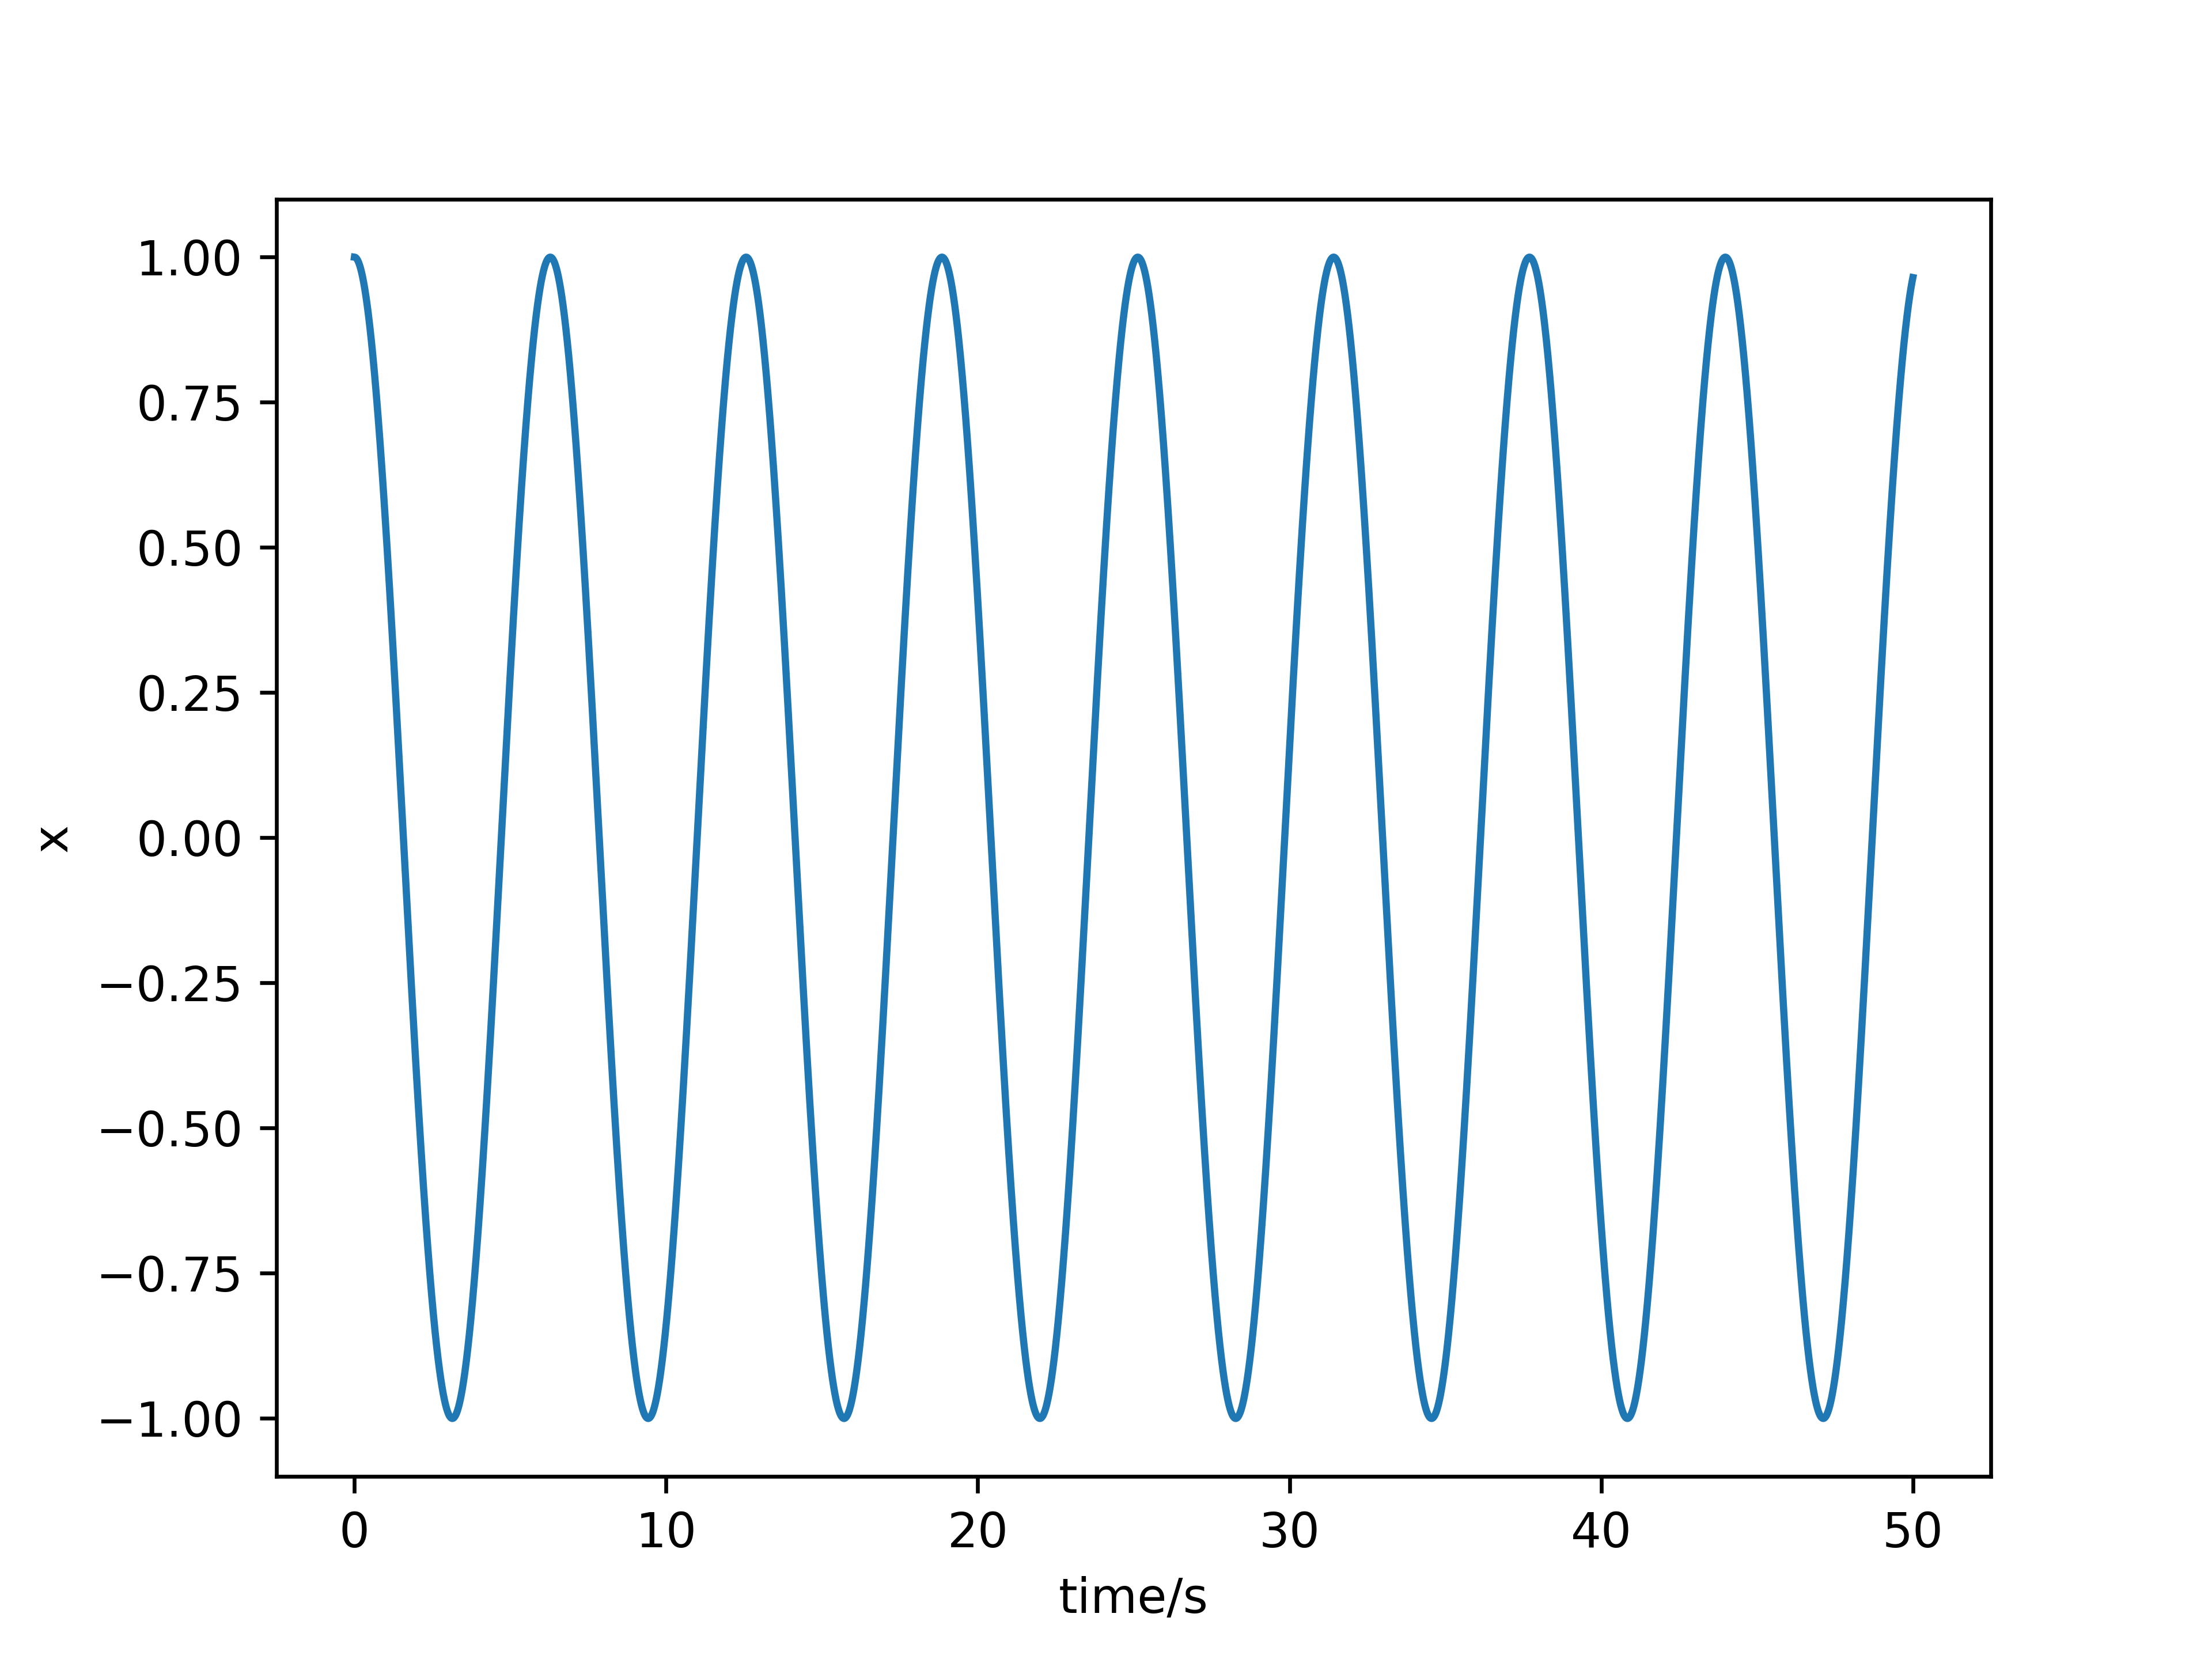
\includegraphics[width=10cm]{9-6a.png}
\end{table}%
\newpage

Then we solve the same problem with different initial position. We found that the system oscillates in same frequency and different amplitude.

\begin{table}[!h]
    \centering
    \caption{x as a function of time for harmonic trap for different amplitude}
    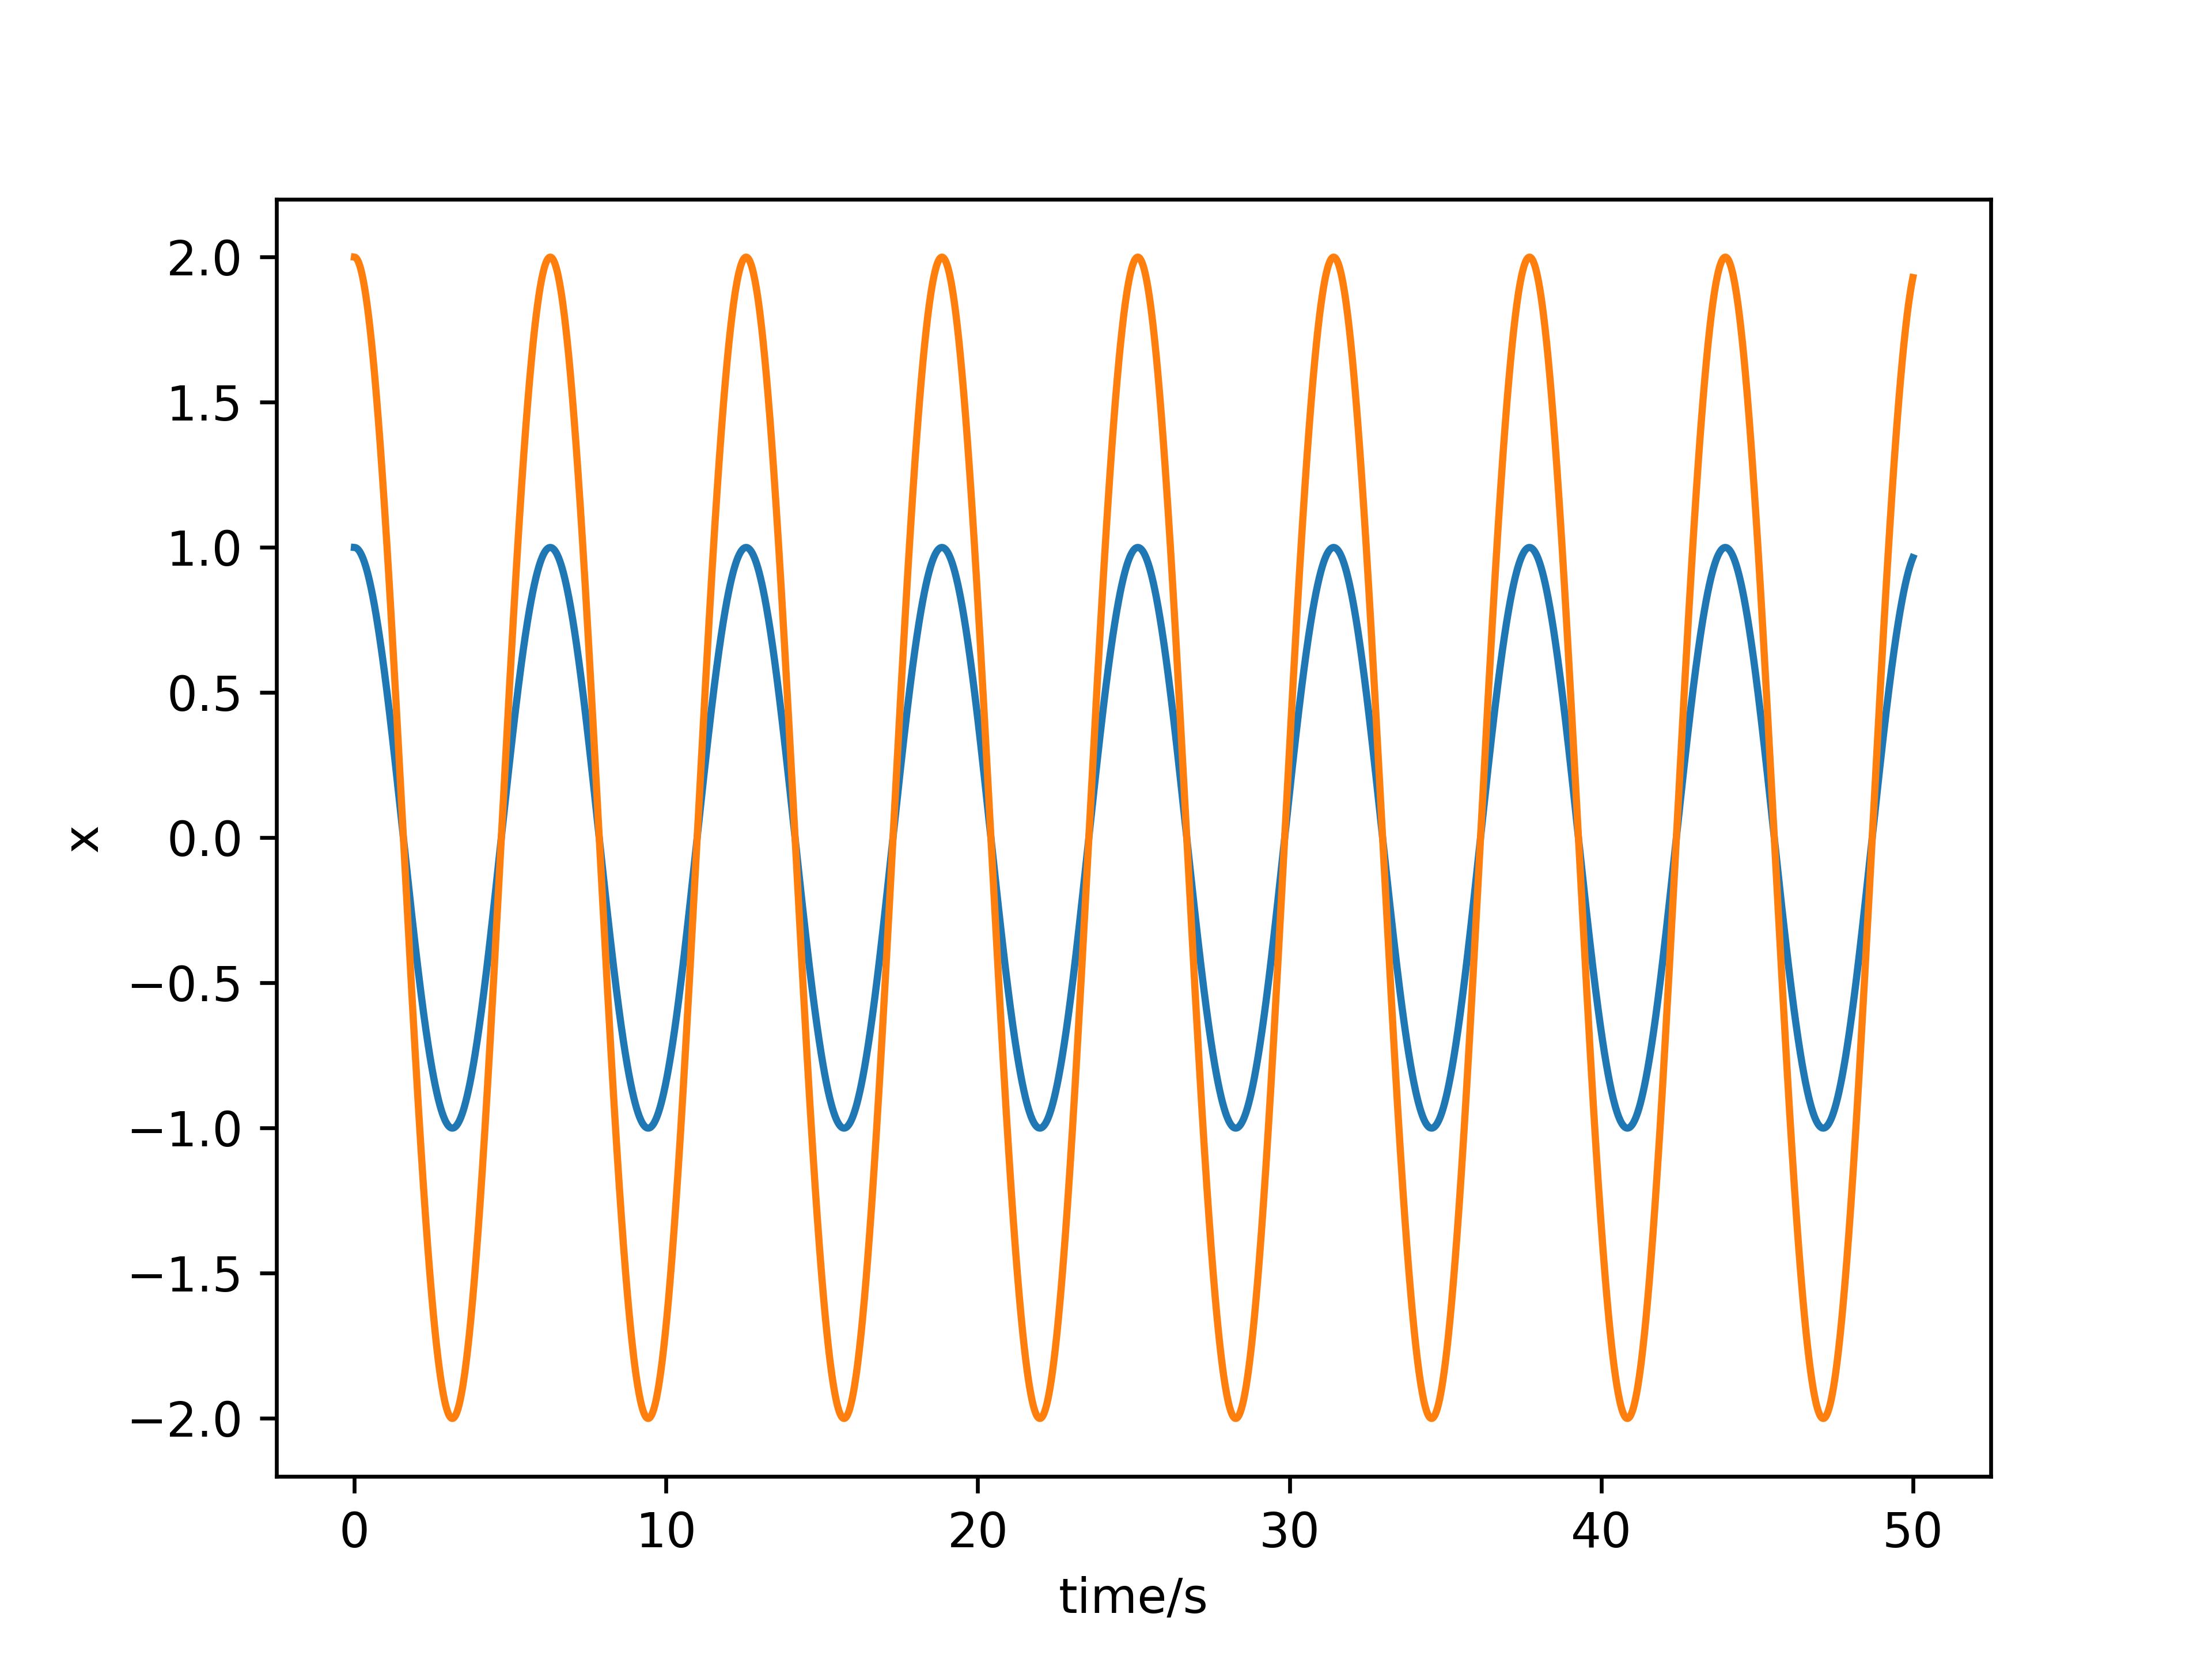
\includegraphics[width=10cm]{9-6b.png}
\end{table}%

Next we solve the anharmonic problem in 9-6c. We plotted the motion of the oscillator for different amplitude. We indeed see that for larger amplitude the system oscillates faster.

\begin{table}[!h]
    \centering
    \caption{x as a function of time for anharmonic trap for different amplitude}
    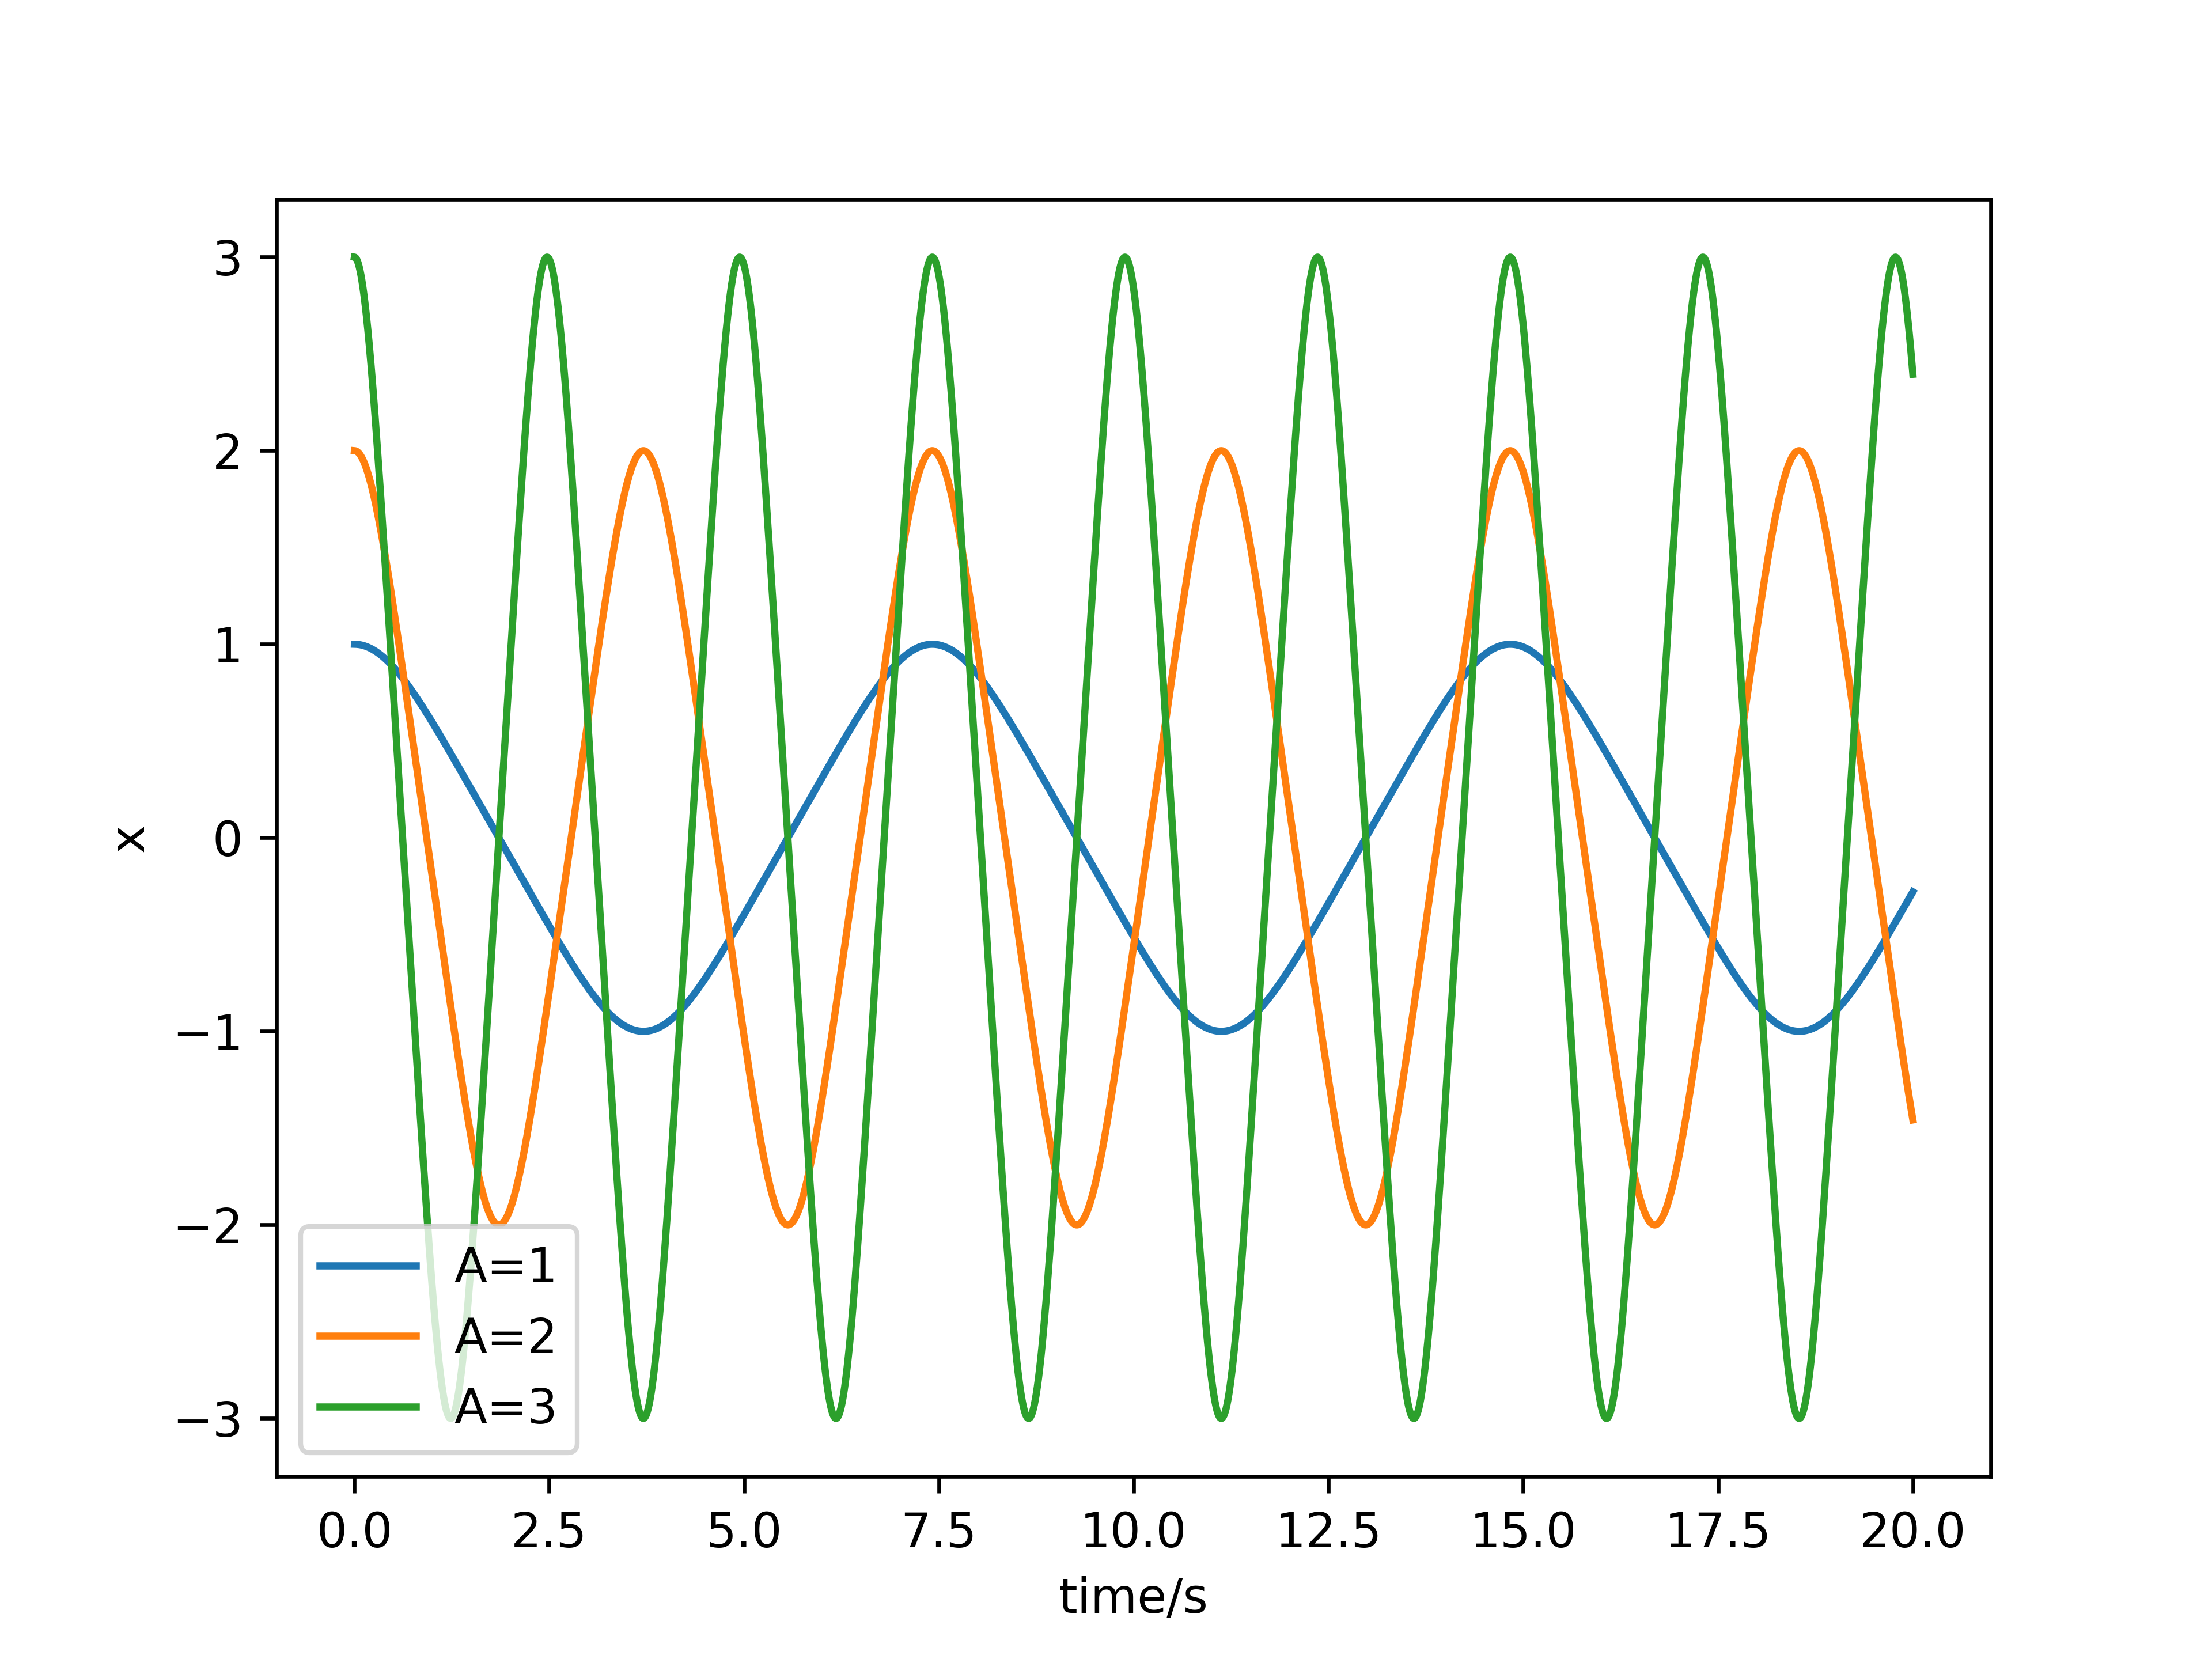
\includegraphics[width=11cm]{9-6c.png}
\end{table}%

Then we plotted the phase space diagram for both harmonic trap and anharmonic trap.

\begin{table}[!h]
    \centering
    \caption{phase space plot for harmonic trap}
    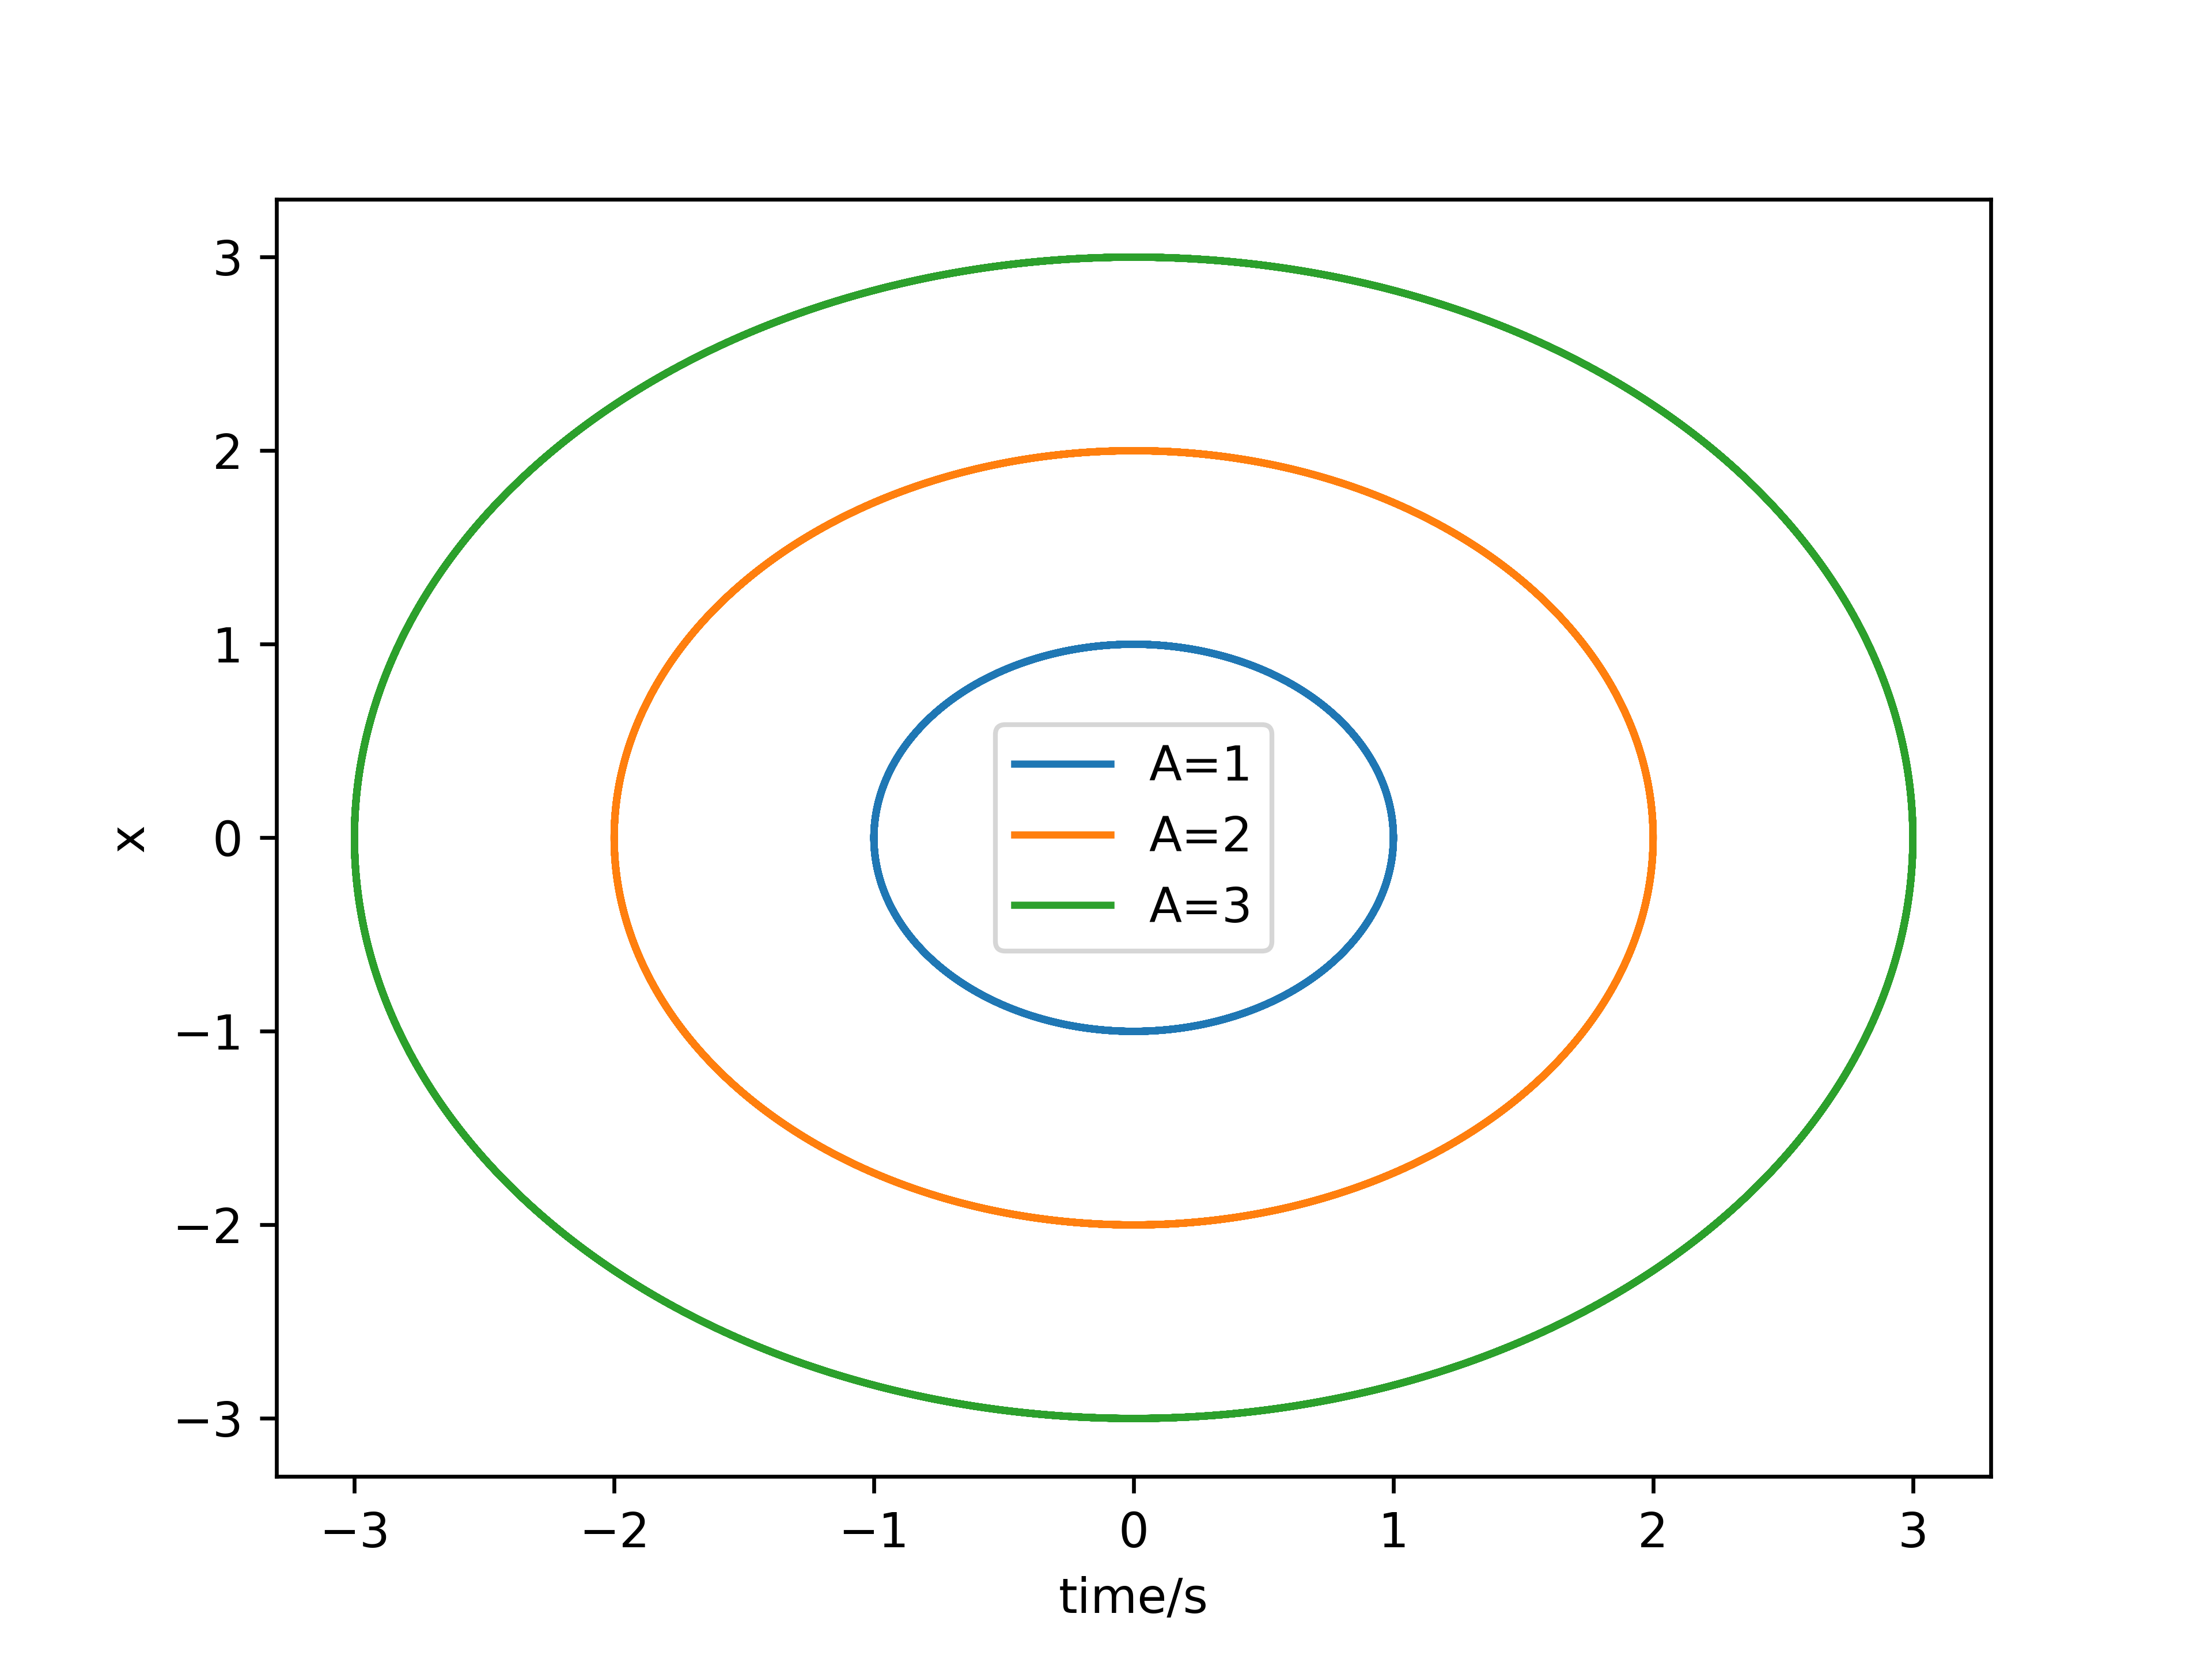
\includegraphics[width=11cm]{9-6d-1.png}
\end{table}%

\begin{table}[!h]
    \centering
    \caption{phase space plot for anharmonic trap}
    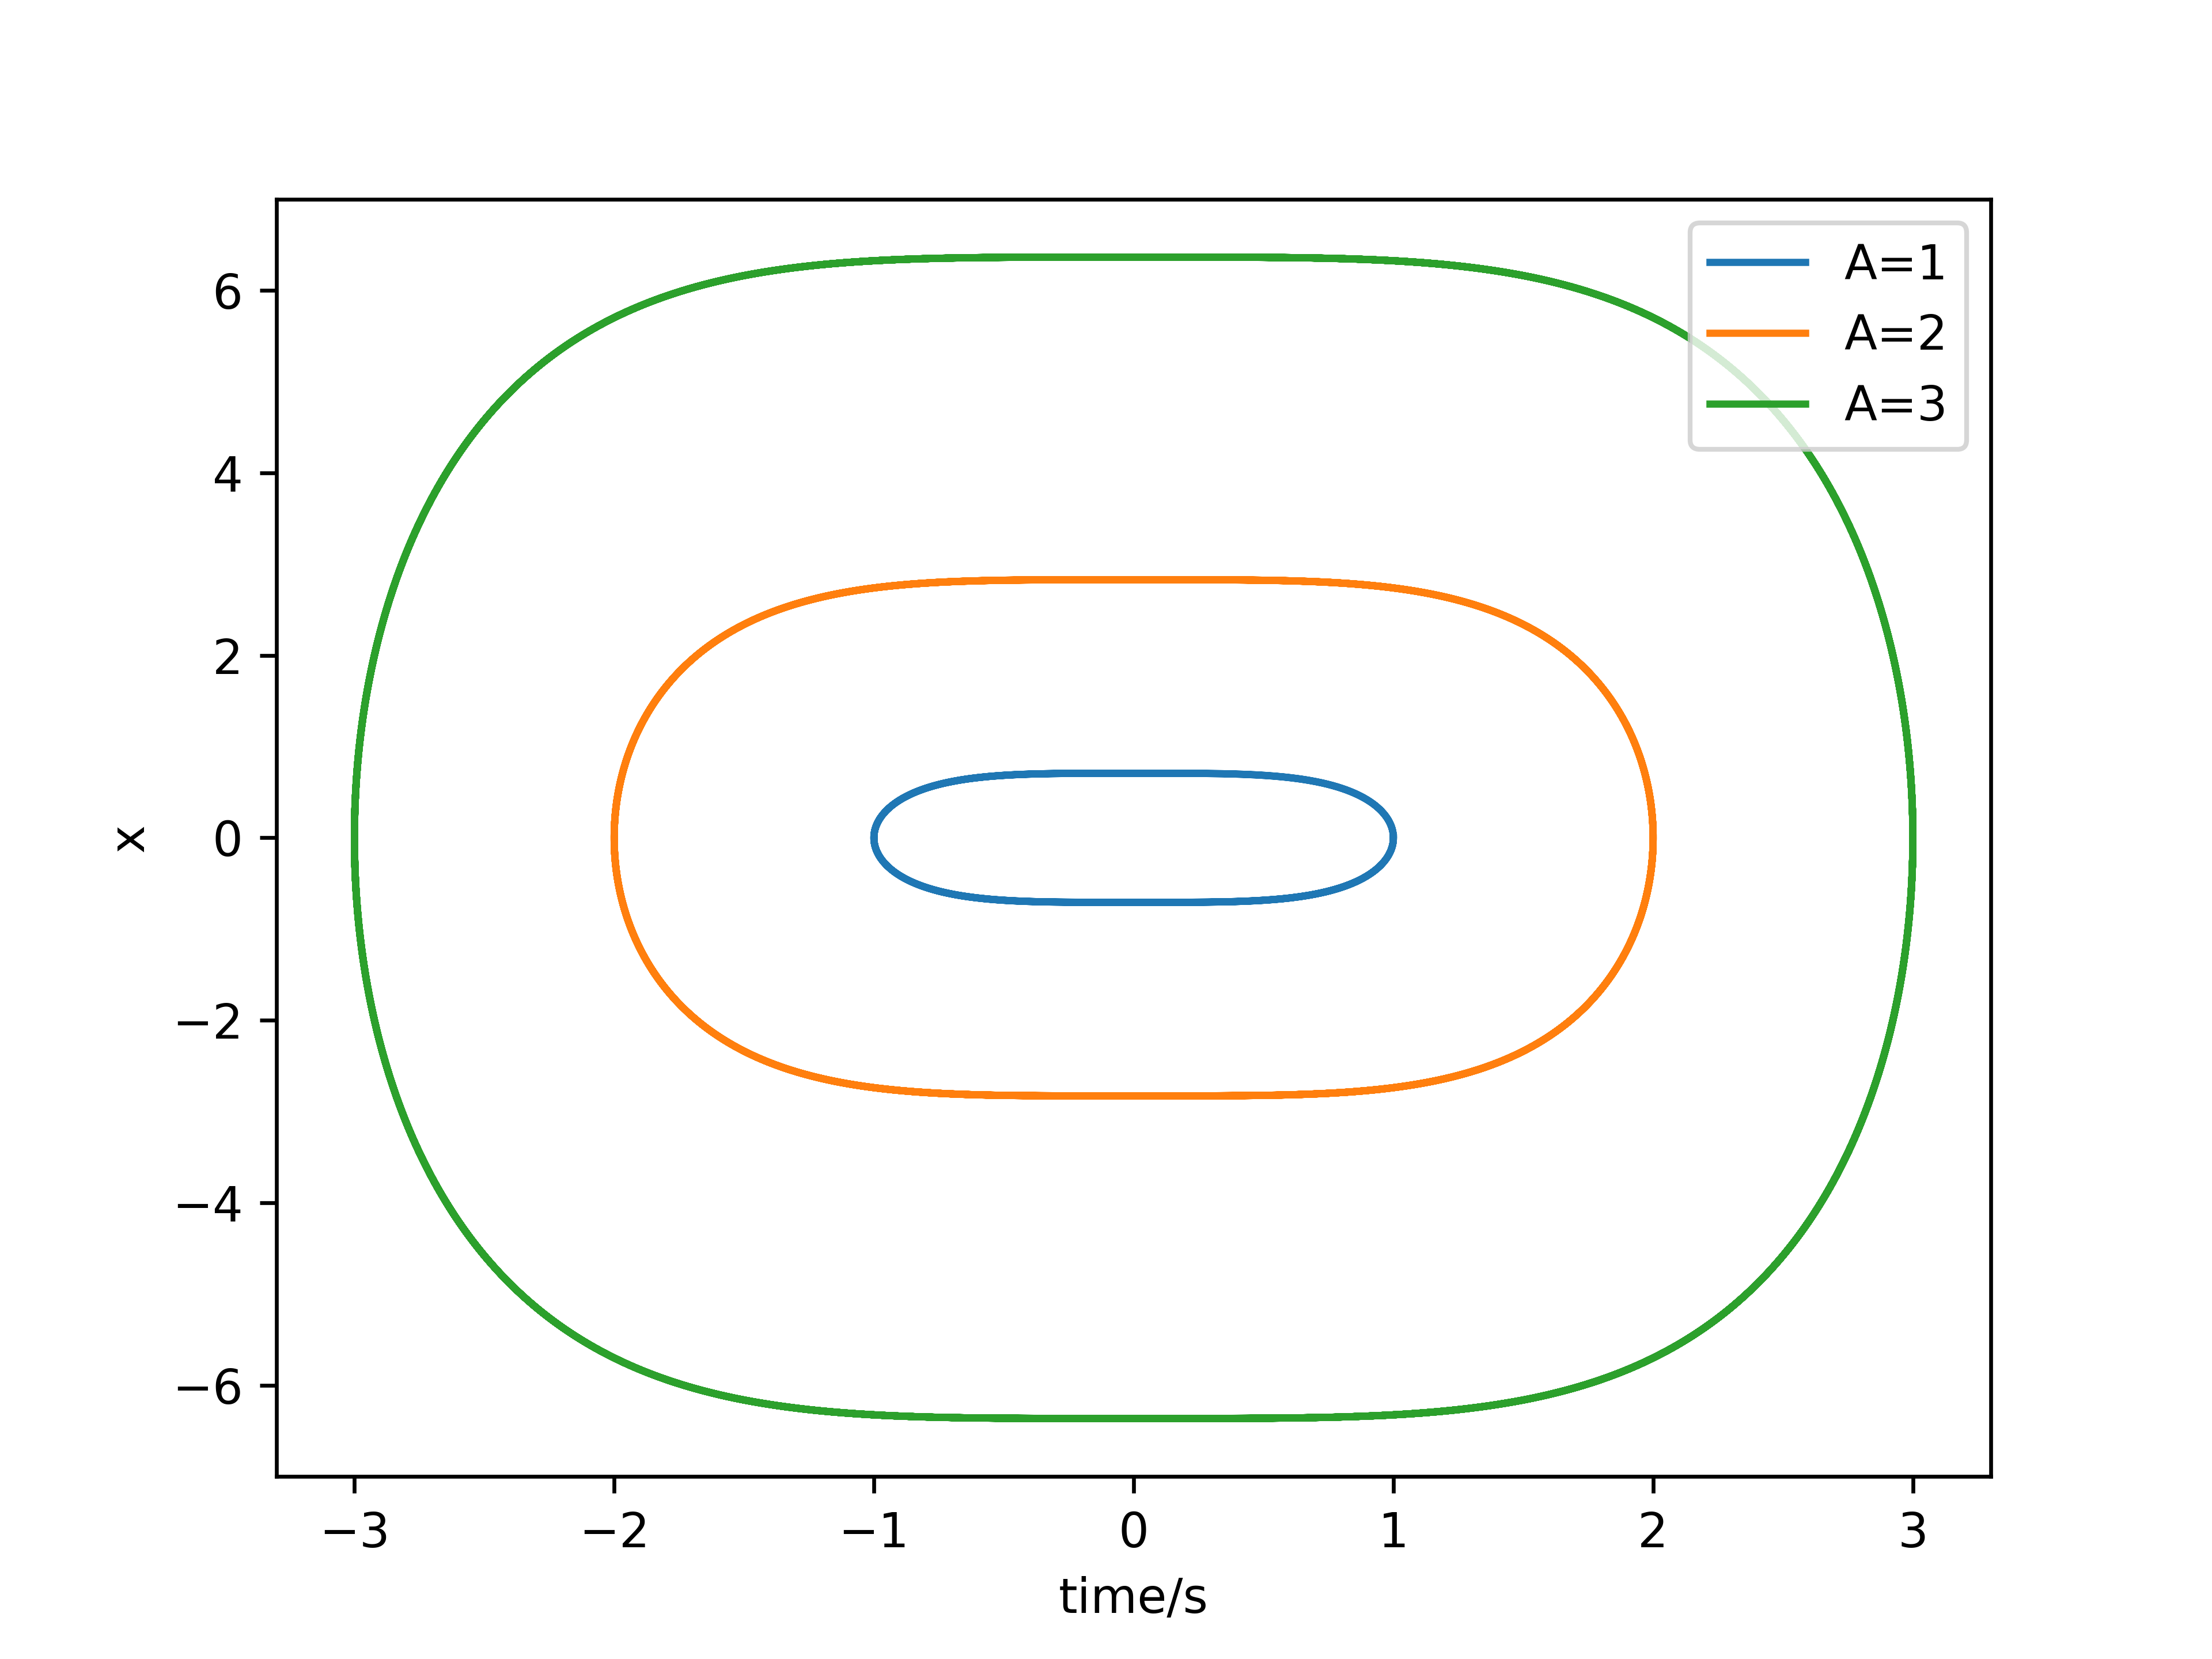
\includegraphics[width=11cm]{9-6d-2.png}
\end{table}%
\newpage

Finally, we solve the equation for van der Pols potential with different $\mu$. Here's the phase space plot.

\begin{table}[!h]
    \centering
    \caption{phase space plot for van der Pols potential}
    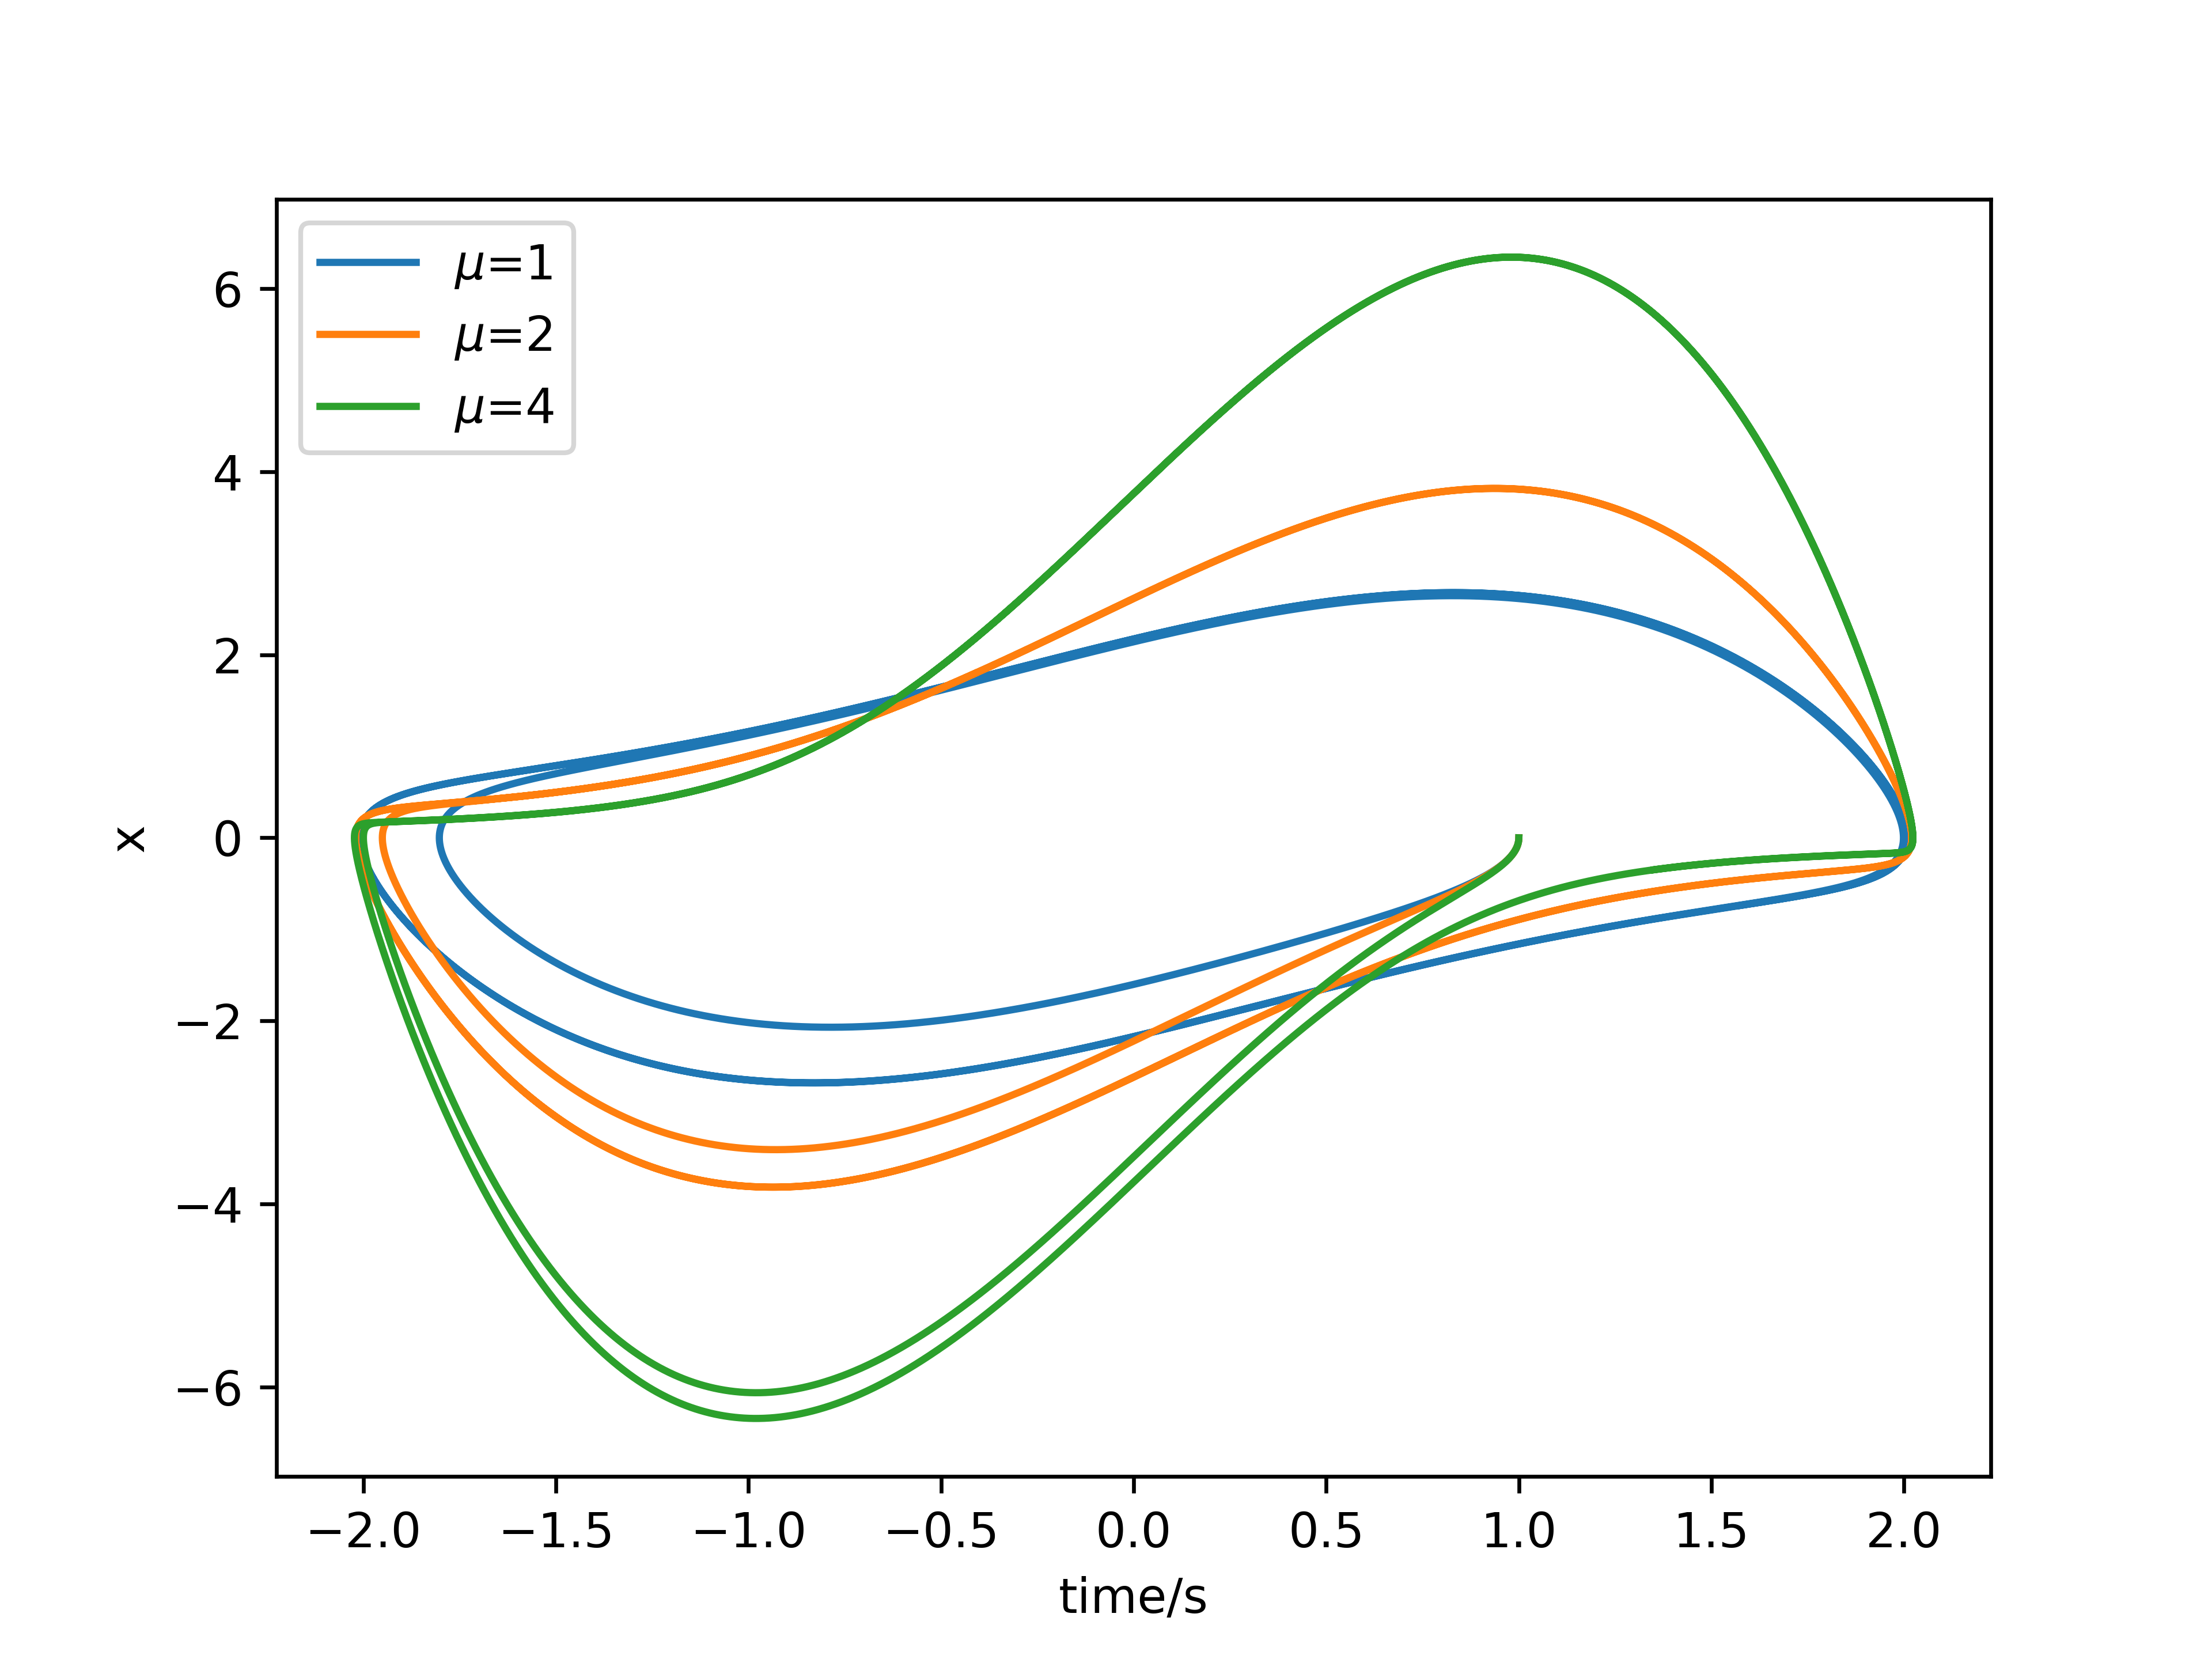
\includegraphics[width=11cm]{9-6e.png}
\end{table}%



\section{Newman 8.7: Trajectory with air resistance}

the associated code can be found in 9-2.py.

The equation of motion for the cannonball is:

\begin{equation}
    m\frac{d^2\vec{x}}{dt^2} = -\frac{1}{2} \pi R^2\rho C \frac{d\vec{x}}{dt}^2 + mg
\end{equation}

So:

\begin{equation}
    \frac{d^2\vec{x}}{dt^2} = -\frac{\pi}{2} \frac{R^2\rho C}{m} \frac{d\vec{x}}{dt}^2 + g
\end{equation}

we first define a typical length $x_0 = \frac{m}{R^2\rho C}$, then the equation of motion becomes:

\begin{equation}
    \frac{d^2\vec{x}}{dt^2} = -\frac{\pi}{2} x_0 \frac{d\vec{x}}{dt}^2 + g
\end{equation}

By defining the dimensionless parameter $x' = x/x0$, we have:

\begin{equation}
    \frac{d^2\vec{x'}}{dt^2} = -\frac{\pi}{2} \frac{d\vec{x'}}{dt}^2 + g/x_0
\end{equation}

We can then define a new typical time $T_0^2 = x_0/g = R^2 \rho C g/m$, and $t' = t/T_0$ we have the equation of motion:

\begin{equation}
    \frac{d^2\vec{x'}}{dt'^2} = -\frac{\pi}{2} \frac{d\vec{x'}}{dt'}^2 + 1
\end{equation}

The total equation of motion can be extracted by rescaling variables $t'$ and $x'$, which is on a one dimension manifold.

Now we derive the equation of motion in x and y direction. With the resistance force $F_{air} = -\frac{\pi}{2} \rho C R^2 v^2$ We have:

\begin{align}
    & m\ddot{x} = -F_{air} \frac{\dot{x}}{\sqrt{\dot{x}^2 + \dot{y}^2}}\\
    & m\ddot{y} = -F_{air} \frac{\dot{y}}{\sqrt{\dot{x}^2 + \dot{y}^2}} - mg
\end{align}

After taking in the explicit form of air resistance force, we have the equation of motion:

\begin{align}
    & \ddot{x} = -\frac{\pi}{2m} \rho C R^2 v^2 \frac{\dot{x}}{\sqrt{\dot{x}^2 + \dot{y}^2}}\\
    & \ddot{y} = -\frac{\pi}{2m} \rho C R^2 v^2 \frac{\dot{y}}{\sqrt{\dot{x}^2 + \dot{y}^2}} - g
\end{align}

We know that $v^2 = \dot{x}^2 + \dot{y}^2$

\begin{align}
    & \ddot{x} = -\frac{\pi R^2 \rho C}{2m}   \sqrt{\dot{x}^2 + \dot{y}^2} \dot{x}\\
    & \ddot{y} = -\frac{\pi R^2 \rho C}{2m}   \sqrt{\dot{x}^2 + \dot{y}^2} \dot{y} - g
\end{align}

We carried out the calculation numerically and here's the trajectory with parameters in Newman's book(with 100m/s initial velocity shot at 30 degree from horizontal):

\begin{table}[!h]
    \centering
    \caption{trajectory for cannonball with air resistance}
    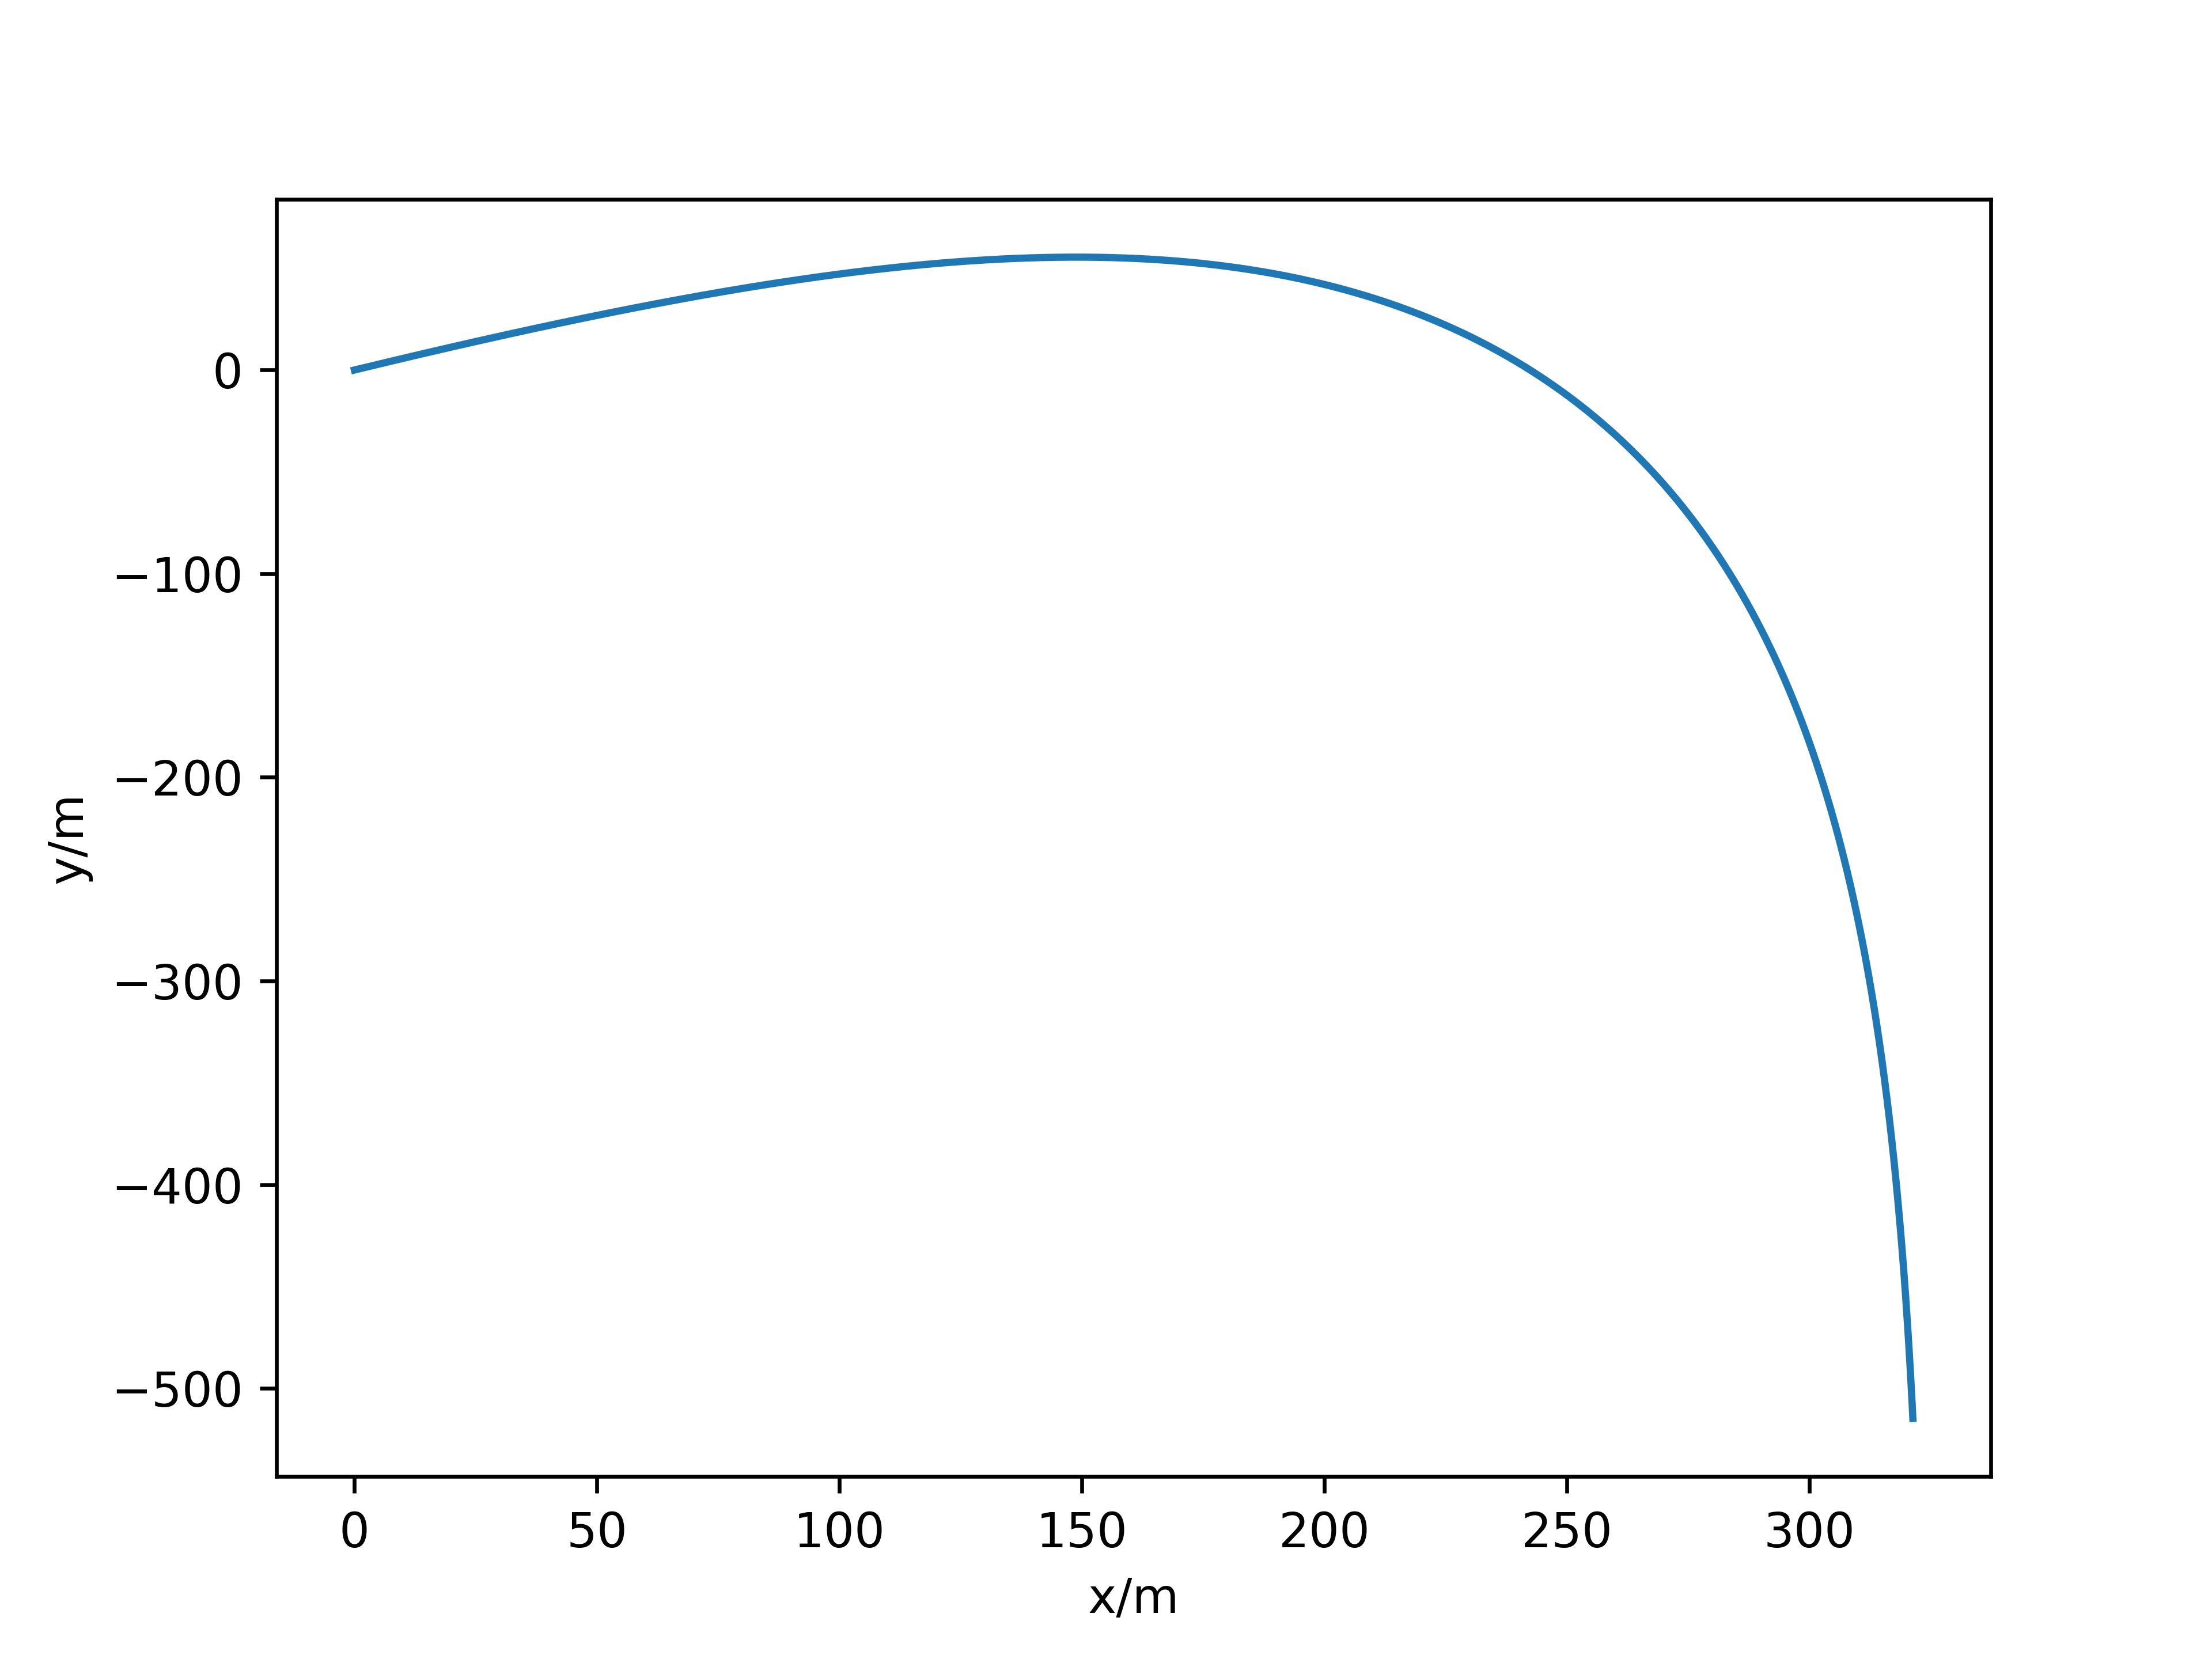
\includegraphics[width=10cm]{9-7b.png}
\end{table}%
\newpage

Next, we carried out the calculation for launching cannonball with different mass but same shape and same initial velocity. Here's our calculation result:

\begin{table}[!h]
    \centering
    \caption{trajectory for cannonball with air resistance}
    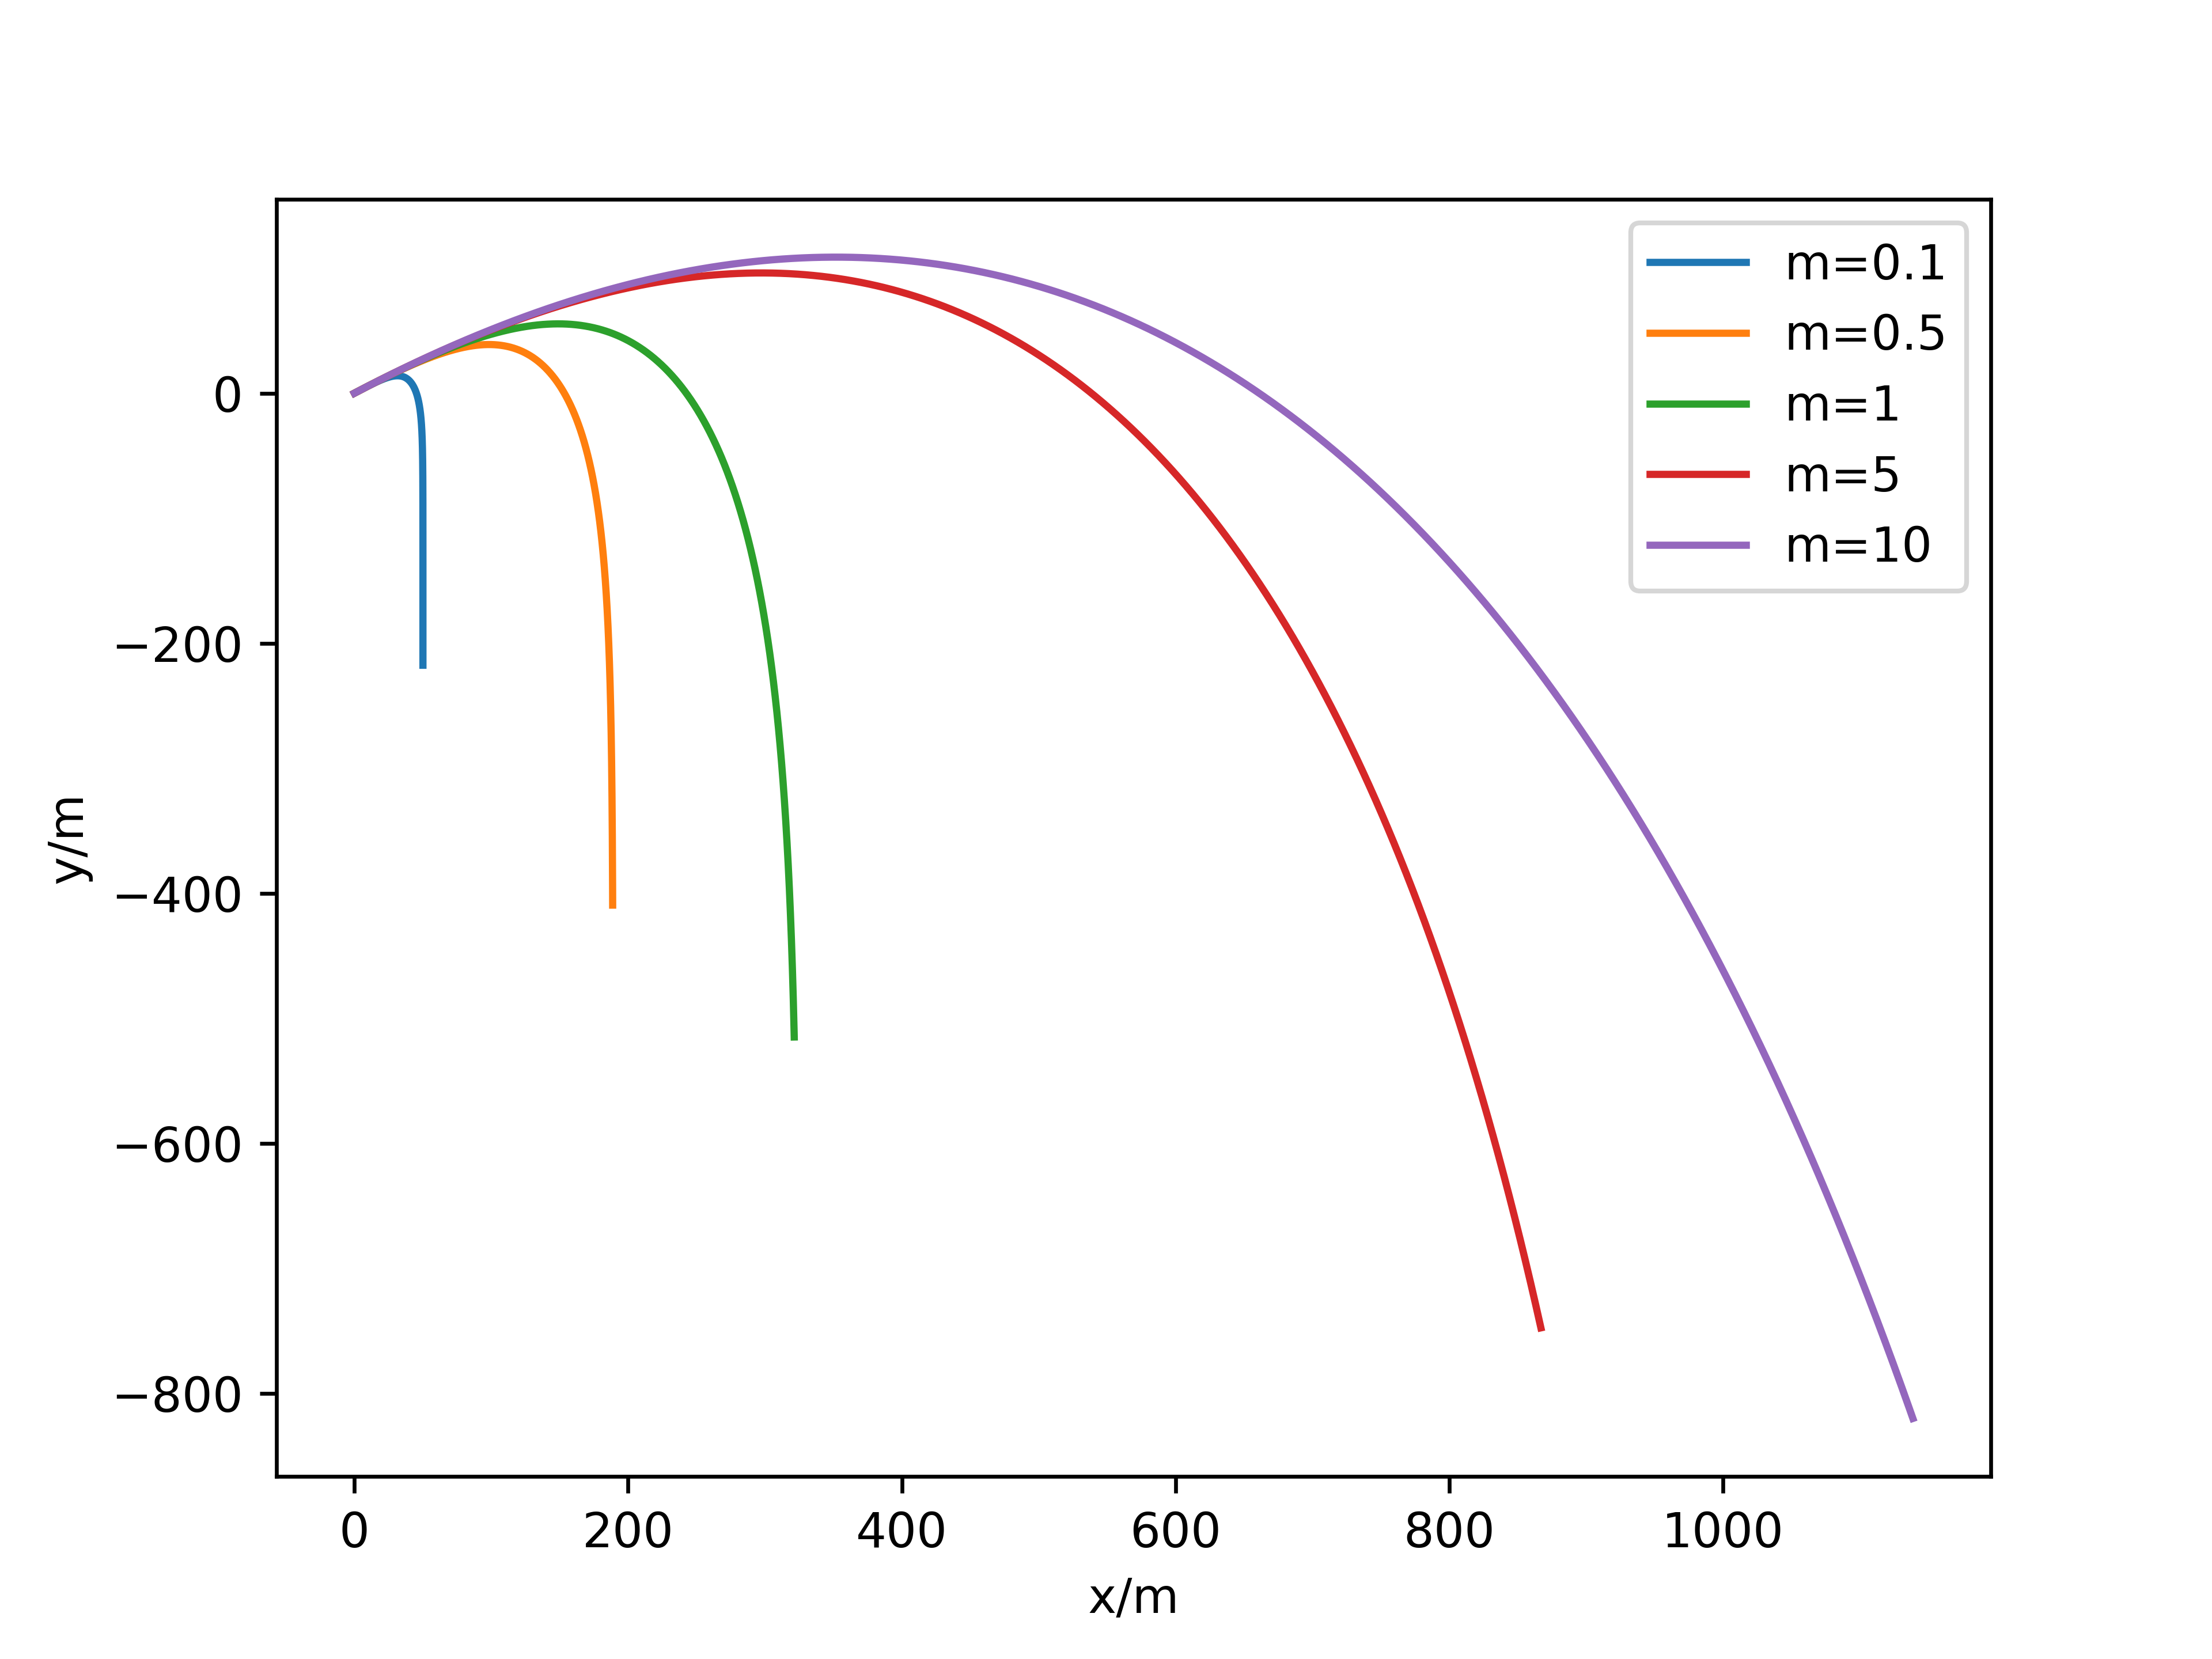
\includegraphics[width=10cm]{9-7c.png}
\end{table}%

We found out that the higher the mass, the further the cannonball can go to. This is basically because that, for cannonball with larger mass, the resistance force from air is relatively weaker. The cannonball thus can go further.





\end{document}